\documentclass[letterpaper]{article}
\usepackage[margin=1in]{geometry}
\usepackage[utf8]{inputenc}
\usepackage{textcomp}
\usepackage{amssymb}
\usepackage{natbib}
\usepackage{graphicx}
\usepackage{gensymb}
\usepackage{amsthm, amsmath, mathtools}
\usepackage[dvipsnames]{xcolor}
\usepackage{enumerate}
\usepackage{mdframed}
\usepackage[most]{tcolorbox}
\usepackage{csquotes}
% https://tex.stackexchange.com/questions/13506/how-to-continue-the-framed-text-box-on-multiple-pages

\tcbuselibrary{theorems}

\newcommand{\R}{\mathbb{R}}
\newcommand{\Z}{\mathbb{Z}}
\newcommand{\N}{\mathbb{N}}
\newcommand{\Q}{\mathbb{Q}}
\newcommand{\C}{\mathbb{C}}
\newcommand{\code}[1]{\texttt{#1}}
\newcommand{\mdiamond}{$\diamondsuit$}
\newcommand{\PowerSet}{\mathcal{P}}
\newcommand{\Mod}[1]{\ (\mathrm{mod}\ #1)}
\DeclareMathOperator{\lcm}{lcm}

%\newtheorem*{theorem}{Theorem}
%\newtheorem*{definition}{Definition}
%\newtheorem*{corollary}{Corollary}
%\newtheorem*{lemma}{Lemma}
\newtheorem*{proposition}{Proposition}


\newtcbtheorem[number within=section]{theorem}{Theorem}
{colback=green!5,colframe=green!35!black,fonttitle=\bfseries}{th}

\newtcbtheorem[number within=section]{definition}{Definition}
{colback=blue!5,colframe=blue!35!black,fonttitle=\bfseries}{def}

\newtcbtheorem[number within=section]{corollary}{Corollary}
{colback=yellow!5,colframe=yellow!35!black,fonttitle=\bfseries}{cor}

\newtcbtheorem[number within=section]{lemma}{Lemma}
{colback=red!5,colframe=red!35!black,fonttitle=\bfseries}{lem}

\newtcbtheorem[number within=section]{example}{Example}
{colback=white!5,colframe=white!35!black,fonttitle=\bfseries}{def}

\newtcbtheorem[number within=section]{note}{Important Note}{
        enhanced,
        sharp corners,
        attach boxed title to top left={
            xshift=-1mm,
            yshift=-5mm,
            yshifttext=-1mm
        },
        top=1.5em,
        colback=white,
        colframe=black,
        fonttitle=\bfseries,
        boxed title style={
            sharp corners,
            size=small,
            colback=red!75!black,
            colframe=red!75!black,
        } 
    }{impnote}
\usepackage[utf8]{inputenc}
\usepackage[english]{babel}
\usepackage{fancyhdr}
\usepackage[hidelinks]{hyperref}

\pagestyle{fancy}
\fancyhf{}
\rhead{CSE 131}
\chead{Friday, May 05, 2023}
\lhead{Lecture 15}
\rfoot{\thepage}

\setlength{\parindent}{0pt}

\begin{document}

\section{Structured Data: Pairs (Continued)}
In this section, we'll discuss more about structured data, in particular \textbf{pairs}.

\subsection{Heap Allocation}
We actually have two things we need to do here: 
\begin{itemize}
    \item We need to create some sort of a \emph{heap} that our compiler can use to store pair values. Once we create 
    \item We need to put the heap pointer into \code{r15}.
\end{itemize}
Let's think about some ideas for how we can set the heap up.
\begin{itemize}
    \item One idea is to set \code{r15} to \verb|rsp - {a lot}|. In other words, if we move \code{rsp} very high up, then we can use \code{r15} as the ``heap'' pointer. \textbf{However}, let's think about the process layout:
    \begin{center}
        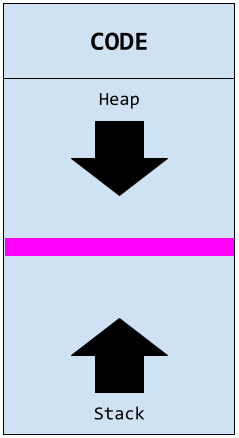
\includegraphics[scale=0.4]{../assets/process_layout.png}
    \end{center}
    The typical convention is that the heap grows downwards and the stack grows upwards. In around the middle of memory (denoted by the pink rectangle), there's some special addresses where touching them will result in an error (heap overflows and stack overflows). So, if we set \code{rsp} high enough, then we might either hit that special address, or if we have a depth-heavy recursion\footnote{Since this can hit our proposed ``heap'' space.}, or if we somehow point \code{r15} to the heap space\footnote{Since this is where Rust might allocate memory, so we might end up overwriting memory that Rust needs.}, then we'll be in trouble. 

    \item We can also call Rust's equivalent of \code{malloc}, and use its value\footnote{\code{malloc} gives us the address to some allocated memory in the heap.}. In particular, 
    \begin{itemize}
        \item Call \code{malloc} for each pair\footnote{Note that heap size is \emph{unknowable} iin general \textbf{statically}.}, or 
        \item One \emph{big} \code{malloc}.
    \end{itemize}
    The suggestion we'll use is similar to having a \textbf{big} \code{malloc}. This has the added benefit of being easy to \code{free} at the end. 
\end{itemize}

\subsection{Modifying Our Rust Code}
Now, we need to modify our Rust code to account for these changes. 

\subsubsection{Modifying the Runtime}
In \code{runtime.rs}, we'll essentially do the following:
\begin{verbatim}
    fn main() {
        let args = ...;
        let input = parse_arg(&args);
        let mut memory = Vec::with_capacity(100_000);       // New!
        let buffer: *mut u64 = memory.as_mut_ptr();         // New! 
        let i: i64 = unsafe {
            our_code_starts_here(input, buffer); 
        };

        snek_print(i);
    }\end{verbatim}
Essentially, we'll create a vector with an initial capaity of \code{100\_000} elements. This will represent our heap. Then, we can get a pointer to that vector, and then pass that pointer into our generated assembly. This means our signature for \code{our\_code\_starts\_here} will look like:
\begin{verbatim}
    extern "C" {
        #[link_name = "\x01our_code_starts_here"]
        fn our_code_starts_here(input: i64, buffer: *mut u64) -> i64;
    }\end{verbatim}

\subsubsection{The Generated Assembly}
In our generated assembly, we'll have 
\begin{verbatim}
    our_code_starts_here:
        mov r15, rsi
        ...\end{verbatim}
Here, \code{rsi} represents the \emph{second} argument\footnote{Recall the x86\_64 calling convention.}. 

\subsubsection{Printing Values}
Finally, we need to adjust the \code{snek\_print} function. In particular, our function now needs to account for the fact that it can either receive 
\begin{itemize}
    \item a number (with tag \code{0}).
    \item a boolean (with tag \code{11}).
    \item a pair (with tag \code{01}).
    \item \code{nil} (with tag \code{1}).
\end{itemize}
With this in mind, we have 
\begin{verbatim}
    fn snek_str(val: i64) -> String {
        if val == 7 { "true".to_owned()} 
        else if val == 3 { "false".to_owned() } 
        else if val % 2 == 0 { format!("{}", val >> 1) } 
        else if val == 1 { "nil".to_owned() } 
        else if val & 1 == 1 {
            let addr = (val - 1) as *const i64; 
            let fst = unsafe { *addr };
            let snd = unsafe { *addr.offset(1) };
            format!("(pair {} {})", snek_str(fst), snek_str(snd))
        } else { format!("unknown value: {val}") }
    }

    #[export_name = "\x01snek_print"]
    fn snek_print(val: i64) -> i64 {
        println!("{}", snek_str(val));
        val 
    }\end{verbatim}
Note that \code{offset} is used so we don't need to do direct pointer arithmetic\footnote{We're looking at the memory location directly next to the current memory location since pairs are contiguous.}. Note that we'll need to do some work printing parentheses and whatnot.


\end{document}